\section{Comparing Stochastic Gradient Descent and Recursive Least Squares}

I used the UCI Machine Learning Repository Parkinson's Data Set\footnote{https://archive.ics.uci.edu/ml/datasets/parkinsons} for this analysis.

Using this dataset I will be attempting to predict the UPDRS, a score to rate the severity of symptoms displayed by a subject with Parkinson's. The only data the model will have available are a number of measures of measures of vocal ability displayed by the subject. These measures include maximum, average and mean vocal fundamental frequency, variation in frequency and in amplitude.

There are several features that we are not interested within this dataset, and these must be dropped to avoid the model having any extra features to attempt prediction from. The features that have been dropped include age, sex, test\_time and motor\_UPDRS.
\subsection{Single Subject}
There are 42 subjects features within the dataset, subject 12 was randomly selected to investigate the performance on a single series.

The UPDRS shows a regular cyclic pattern over the span of the measurements. There are only 107 measurements available for this subject, so it will be interesting how RLS compares to SGD as there will only be that many iterations of the algorithm compared to 3000.
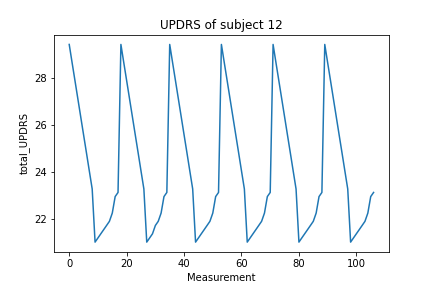
\includegraphics[width=\linewidth]{figs/Parks true single.png}
LinRegSGD\_smoothed was used in order to gently level the error into a single final measurement, rather than allowing for a fluctuating error, learning rate was set to 0.0005 over 300 iterations.
Stochastic Gradient Descent quickly falls to some of it's lowest errors within the first 20 iterations, this rises slowly over iterations 200-2000 before falling slowly back down to a final error per point of 0.312.

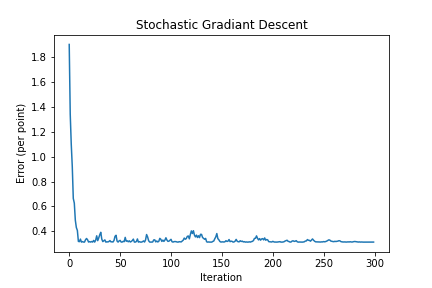
\includegraphics[width=\linewidth]{figs/Parks SGD single.png}

Recursive Least Squares quickly reduces the error over the entire dataset within the first 10 samples given to the model. This error per point has a slight bump before completely converging of it's final score that may be due to the model learning the cyclic pattern in the data.

Interestingly on the plot of error on the data point given the the algorithm at that point, the cyclic pattern of the data can be seen. This may be due to the algorithm initially struggling to capture these cycles and being "surprised" by them every time.
The final error per point from the RLS algorithm with forgetting factor 0.98 is 0.233.

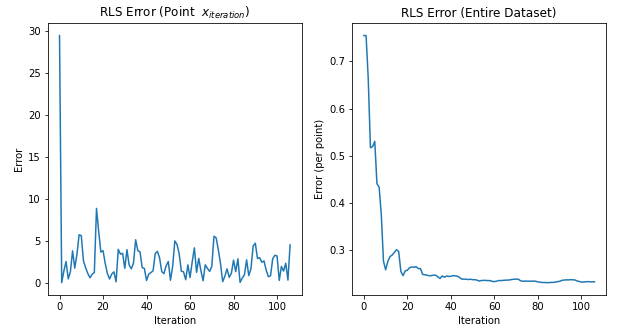
\includegraphics[width=\linewidth]{figs/Parks RLS single.png}
\subsection{All Subjects}
By predicting on all of these subjects independently we can get a much better picture on how these two methods are able to work with this data.
All runs over this dataset use the same parameters as with the single subject analysis.

All of the RLS runs are very similar in nature, with all of them converging to near their final error value within the first 20 iterations. Within these first twenty iterations there appears to be a block of dataset that do not converge to as low an error and the majority which very quickly converge to a similar error. Once the model has converged the error has a very low variance within a single subject.

Within the SGD runs there is one extreme outlier which does not converge until close to 40 iterations. Ignoring this data set all of the other subjects form a tighter grouping, but with more variance inside the single subjects compared to RLS. 

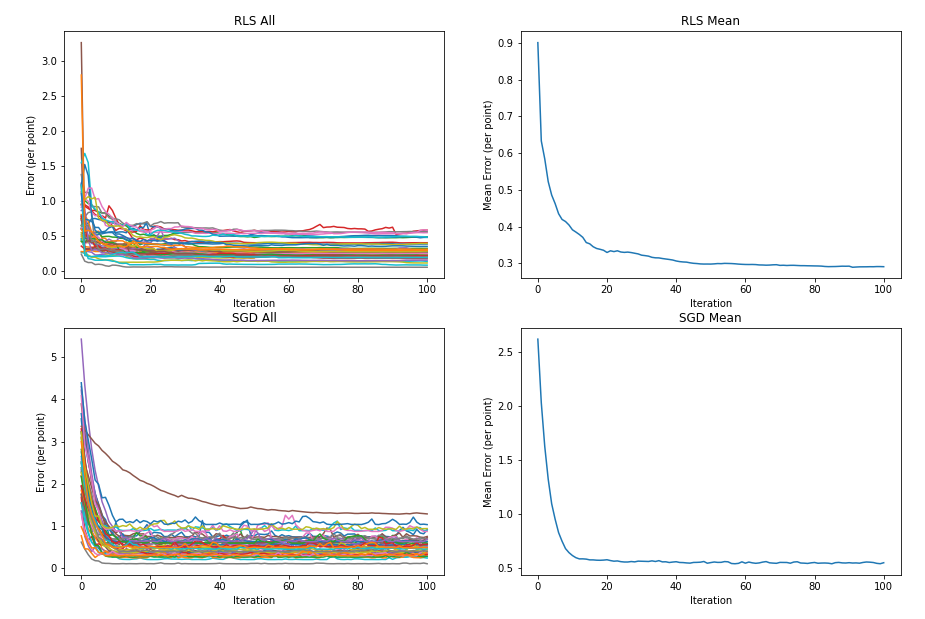
\includegraphics[width=\linewidth]{figs/ParkinsonsALL.png}
To provide easier analysis, all the subject datasets were combined into a single mean for each algorithm. 
The error for SGD falls sharper than RLS, but produces a much less smooth line after this initial convergence. 

The final median error per point for RLS was 0.291 whilst for SGD it was 0.550, RLS was able to converge as fast as SGD while also producing a better error score across the entire set of subjects.